\chapter{Das matérias-primas à reciclagem}\label{ch:g5:raw-materials-and-recycling}

Uma latinha vazia é jogada numa lixeira de \omterm{def:g5:raw-materials-and-recycling:recycling}{reciclagem}. Um caminhão a
leva até um centro de triagem, uma máquina a prensa num bloco junto com
milhares de outras, um forno derrete os blocos e, poucas semanas depois,
o metal está de volta na prateleira de uma loja como uma latinha nova.
De onde veio o metal, para começo de conversa, e por que vale a pena
derreter latinhas velhas em vez de produzir metal novo?

\begin{recall}
Um objeto é uma coisa que podemos ver e tocar; o material dele é aquilo
de que ele é feito --- madeira, metal, vidro, plástico, papel, tecido,
pedra (\cref{ch:g1:materials-around-us}). Numa \omterm{def:g5:irreversible-changes:chemical-change}{transformação química}
aparecem substâncias novas, e não há um caminho simples de volta
(\cref{ch:g5:irreversible-changes}).
\end{recall}

\section{Materiais naturais e materiais fabricados}

\begin{definition}[Materiais naturais e materiais fabricados]\label{def:g5:raw-materials-and-recycling:natural-material}
Um \emph{material natural}\index{material natural} é usado mais ou menos
como é encontrado na natureza, só cortado ou moldado: a madeira, a
pedra, o algodão, a lã, o couro. Um \emph{material
fabricado}\index{material fabricado} é produzido pelas pessoas a partir
de substâncias encontradas na natureza, transformando-as, muitas vezes
com calor e com \omterm{def:g5:irreversible-changes:chemical-change}{transformações químicas}: o vidro, o aço, o alumínio, o
plástico, o papel, o concreto.
\end{definition}

\begin{example}[Duas mesas]\label{ex:g5:raw-materials-and-recycling:tables}
Uma mesa de tábuas de carvalho é feita de um \omterm{def:g5:raw-materials-and-recycling:natural-material}{material natural}: a
madeira só foi serrada, aplainada e colada. Uma mesa com tampo de vidro e
pés de aço é feita de \omterm{def:g5:raw-materials-and-recycling:natural-material}{materiais fabricados}: nem o vidro nem o aço são
encontrados assim na natureza.
\end{example}

\section{As matérias-primas}

\begin{definition}[Matéria-prima e minério]\label{def:g5:raw-materials-and-recycling:raw-material}
Uma \emph{matéria-prima}\index{materia-prima@matéria-prima} é uma substância tirada da
natureza para produzir materiais e objetos: árvores, areia, rochas,
petróleo, algodão, lã. Uma rocha da qual se extrai um metal se chama
\emph{minério}\index{minerio@minério}.
\end{definition}

\begin{example}[De onde vêm os materiais]\label{ex:g5:raw-materials-and-recycling:from}
\begin{itemize}
  \item a madeira e o papel vêm das árvores;
  \item o vidro vem da areia, aquecida a uma temperatura muito alta com
        barrilha e calcário;
  \item o ferro e o aço vêm do \omterm{def:g5:raw-materials-and-recycling:raw-material}{minério} de ferro, uma rocha
        avermelhada;
  \item o alumínio vem da bauxita, outro \omterm{def:g5:raw-materials-and-recycling:raw-material}{minério};
  \item a maioria dos plásticos vem do petróleo, bombeado do subsolo;
  \item o algodão vem de uma planta, a lã vem das ovelhas.
\end{itemize}
\end{example}

\begin{omfigure}
\begin{minipage}[b]{0.48\linewidth}\centering
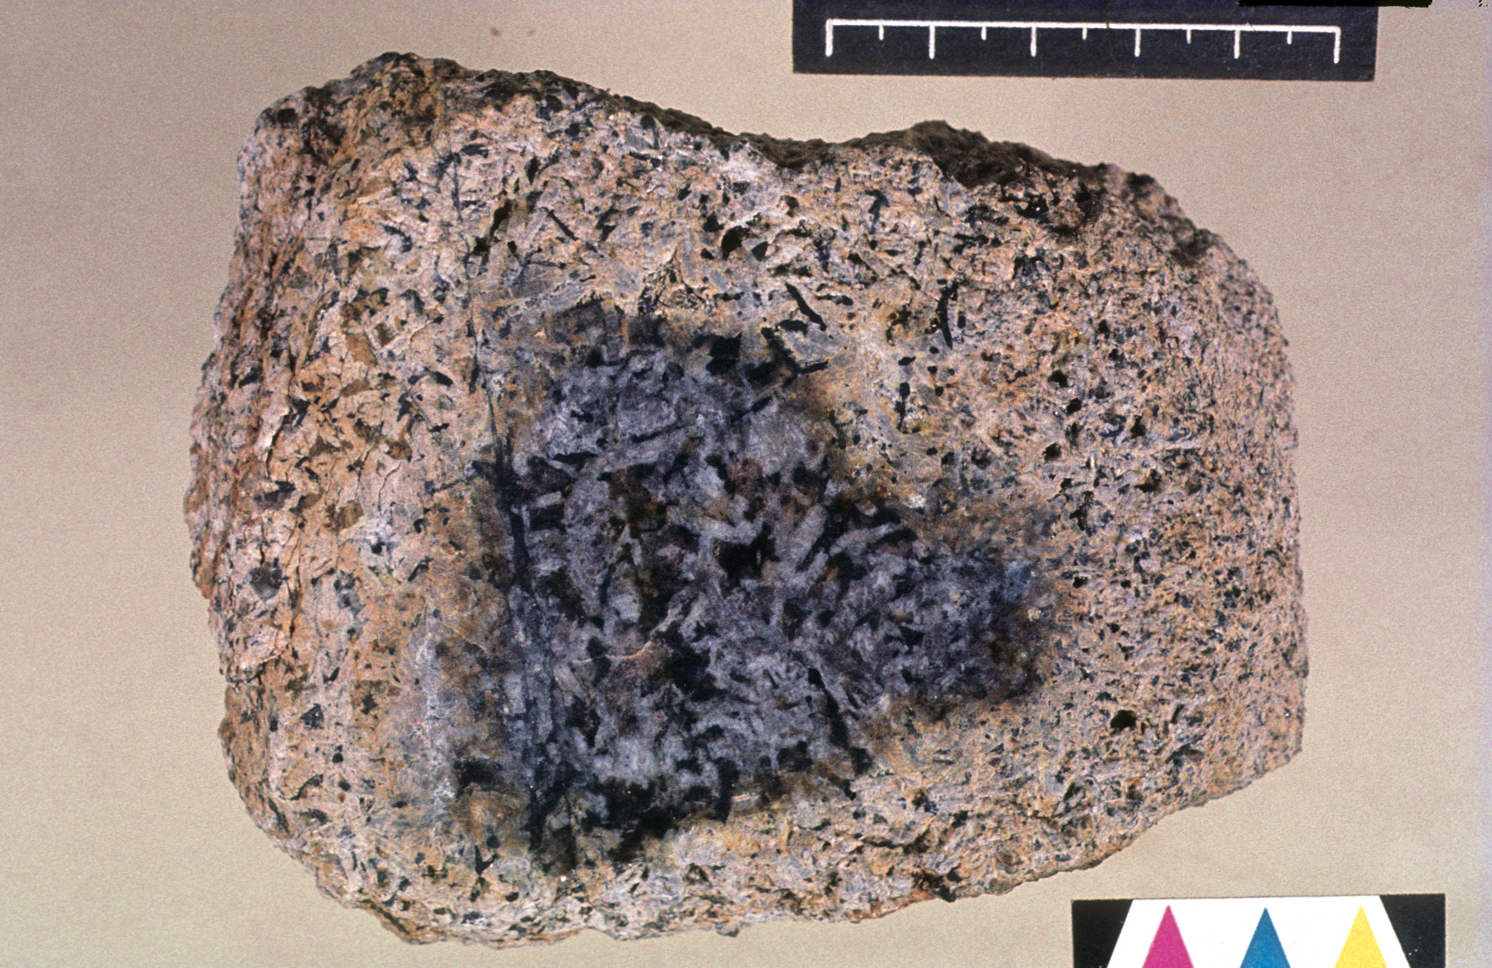
\includegraphics[width=\linewidth,height=4.6cm,keepaspectratio]{images/book1/bauxite.jpg}

{\small A bauxita, o \omterm{def:g5:raw-materials-and-recycling:raw-material}{minério} do alumínio, em volta de um núcleo de rocha
não alterada. Foto: Werner Schellmann, CC BY-SA 2.5.}
\end{minipage}\hfill
\begin{minipage}[b]{0.48\linewidth}\centering
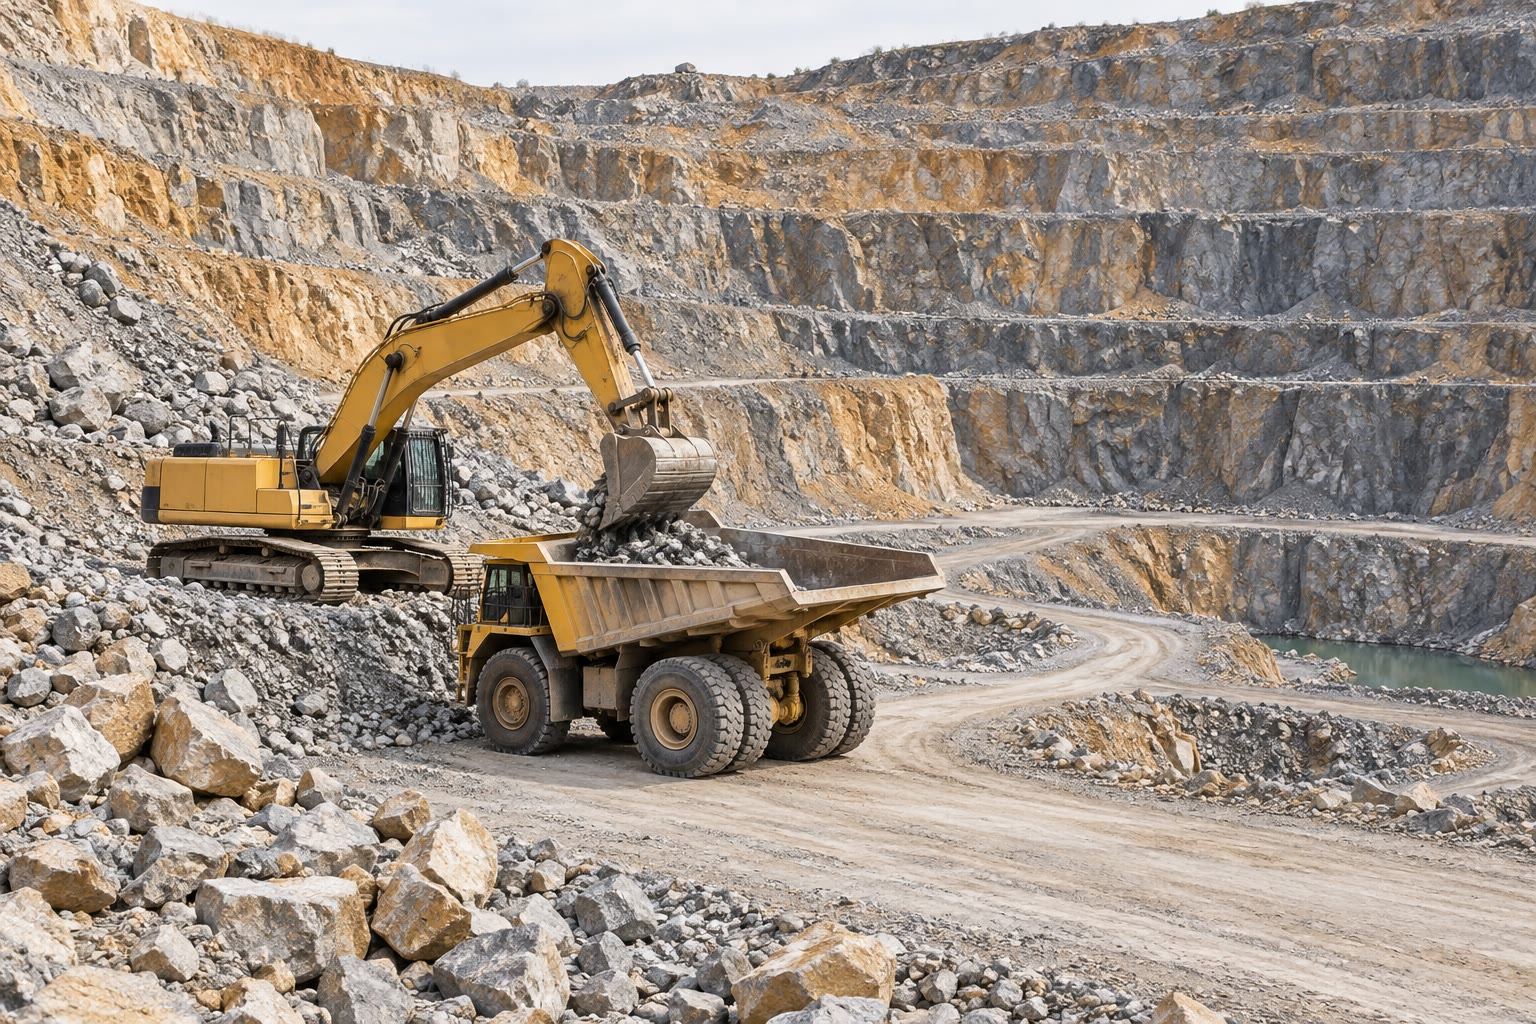
\includegraphics[width=\linewidth,height=4.6cm,keepaspectratio]{images/book1/ai/g5-quarry.jpg}

{\small Uma pedreira: a rocha é extraída para ser usada como \omterm{def:g5:raw-materials-and-recycling:raw-material}{matéria-prima}.}
\end{minipage}
\end{omfigure}

\begin{omfigure}
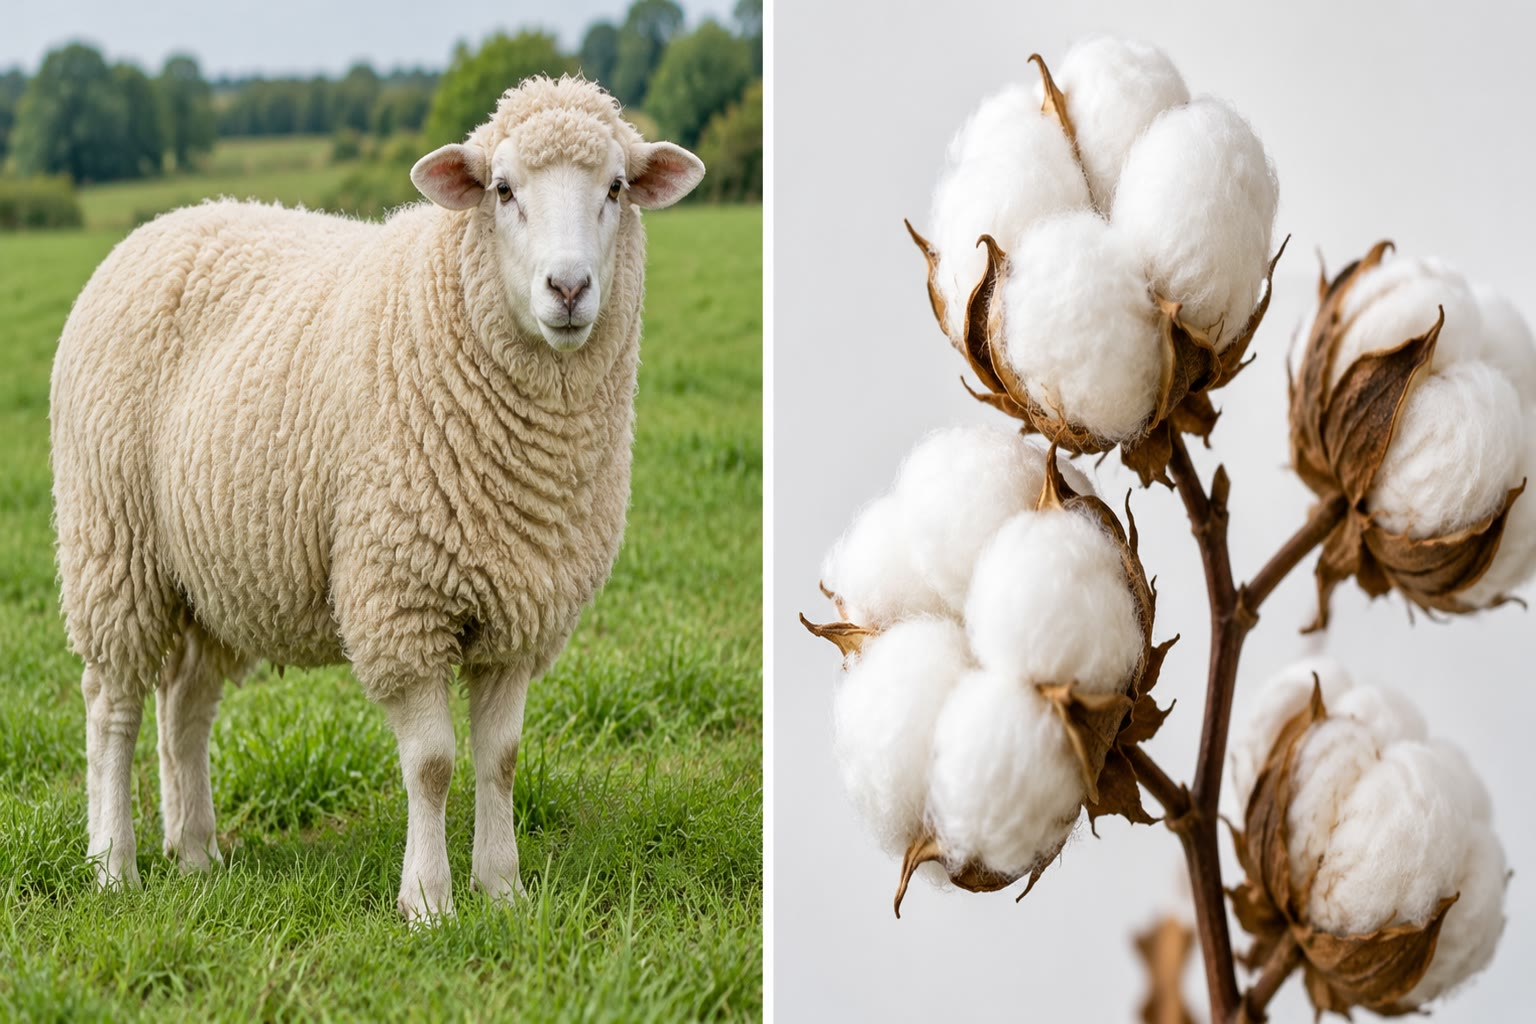
\includegraphics[width=0.6\linewidth]{images/book1/ai/g5-sheep-cotton.jpg}

{\small Matérias-primas naturais que vêm de seres vivos: a lã das
ovelhas, o algodão do algodoeiro.}
\end{omfigure}

\section{Da matéria-prima ao objeto}

\begin{proposition}[Produzir um material transforma a matéria-prima]\label{prop:g5:raw-materials-and-recycling:change}
Transformar uma \omterm{def:g5:raw-materials-and-recycling:raw-material}{matéria-prima} num \omterm{def:g5:raw-materials-and-recycling:natural-material}{material fabricado} exige energia ---
na maioria das vezes, o calor de um forno --- e, em geral,
\omterm{def:g5:irreversible-changes:chemical-change}{transformações químicas}: a areia vira vidro, o \omterm{def:g5:raw-materials-and-recycling:raw-material}{minério} vira metal, o
petróleo vira plástico. Essas transformações não podem ser desfeitas de
um jeito simples: o vidro não volta a ser areia.
\end{proposition}

\begin{example}[A vida de uma garrafa de vidro]\label{ex:g5:raw-materials-and-recycling:bottle}
Areia, barrilha e calcário moído são aquecidos juntos num forno até
derreterem e virarem vidro. O vidro quente é soprado na forma de uma
garrafa. A garrafa é enchida, vendida e esvaziada. Colocada num coletor
de vidro, ela é quebrada em pedacinhos, derretida de novo e soprada numa
garrafa nova: o vidro é usado de novo, muitas e muitas vezes.
\end{example}

\begin{omfigure}
\begin{tikzpicture}[font=\small,
    box/.style={draw=omDef, fill=omDef!6, rounded corners=2pt, align=center,
      minimum height=0.95cm, text width=2.4cm}]
  \node[box] (r) at (0,2.6) {matéria-prima\\ (areia, minério, petróleo)};
  \node[box] (m) at (4.0,2.6) {produção do\\ material};
  \node[box] (o) at (8.0,2.6) {objeto,\\ usado};
  \node[box] (w) at (8.0,0) {lixo};
  \node[box, draw=omProp, fill=omProp!8] (s) at (4.0,0) {triagem e\\ reciclagem};
  \draw[->, thick, omDef] (r) -- (m);
  \draw[->, thick, omDef] (m) -- (o);
  \draw[->, thick, omDef] (o) -- (w);
  \draw[->, thick, omProp] (w) -- (s);
  \draw[->, thick, omProp] (s) -- (m) node[midway, left, align=right, text=black]
    {usado de novo\\ no lugar de\\ matéria-prima nova};
  \draw[->, thick, black!45, dashed] (w.east) -- ++(1.4,0) node[right, align=left,
    text=black] {jogado fora:\\ aterro};
\end{tikzpicture}

{\small A vida de um material. O circuito laranja é a \omterm{def:g5:raw-materials-and-recycling:recycling}{reciclagem}: o
material de um objeto velho substitui uma \omterm{def:g5:raw-materials-and-recycling:raw-material}{matéria-prima} nova.}
\end{omfigure}

\section{Triagem e reciclagem}

\begin{definition}[Reciclagem]\label{def:g5:raw-materials-and-recycling:recycling}
A \emph{reciclagem}\index{reciclagem} consiste em recolher objetos usados
e tratar o material deles para que ele possa virar objetos novos, em vez
de ser jogado fora.
\end{definition}

\begin{proposition}[Por que reciclar]\label{prop:g5:raw-materials-and-recycling:why}
% ledger: al:energy-primary, al:energy-recycled (8.3 / 186 = about 1/22)
A \omterm{def:g5:raw-materials-and-recycling:recycling}{reciclagem} poupa matérias-primas, que não precisam ser extraídas do
subsolo, e muitas vezes poupa energia. Produzir alumínio a partir de
latinhas velhas exige só cerca de um vinte avos da energia necessária
para produzi-lo a partir da bauxita. Ela também significa menos lixo nos
aterros.
\end{proposition}

\begin{method}[Separar o lixo para a reciclagem]\label{met:g5:raw-materials-and-recycling:sort}
A \omterm{def:g5:raw-materials-and-recycling:recycling}{reciclagem} começa com a separação, onde quer que o lixo seja jogado
fora:
\begin{enumerate}
  \item garrafas e potes de vidro num coletor;
  \item latinhas de metal, papel e papelão, e garrafas de plástico nos
        coletores que a cidade oferece para eles (as cores dos coletores
        mudam de um lugar para outro);
  \item o que não pode ser reciclado, com o resto do lixo.
\end{enumerate}
Cada material é reciclado do seu próprio jeito, por isso um coletor só
pode receber os materiais a que ele se destina.
\end{method}

\begin{omfigure}
\begin{tikzpicture}[font=\small]
  \foreach \k/\t/\bc in {0/vidro/green!50!black, 1/{latas de metal}/gray,
                        2/{papel e papelão}/omDef, 3/{garrafas de plástico}/orange!80!black} {
    \begin{scope}[xshift=\k*3.4cm]
      \fill[\bc!18, draw=\bc, line width=0.8pt] (-1,0) -- (1,0) -- (1.15,2.0)
        -- (-1.15,2.0) -- cycle;
      \fill[\bc!45, draw=\bc] (-1.25,2.0) rectangle (1.25,2.3);
      \node[anchor=north, align=center] at (0,-0.15) {\t};
    \end{scope}
  }
  % glass: a bottle
  \fill[green!40!black!60] (-0.2,0.3) rectangle (0.2,1.2);
  \fill[green!40!black!60] (-0.07,1.2) rectangle (0.07,1.6);
  % metal: a can
  \begin{scope}[xshift=3.4cm]
    \fill[black!25, draw=black!55] (-0.3,0.3) rectangle (0.3,1.3);
  \end{scope}
  % paper: a box and a sheet
  \begin{scope}[xshift=6.8cm]
    \fill[brown!25, draw=brown!60] (-0.6,0.3) rectangle (0.1,1.0);
    \fill[white, draw=black!40] (0.2,0.3) rectangle (0.65,1.3);
  \end{scope}
  % plastic: a bottle
  \begin{scope}[xshift=10.2cm]
    \fill[cyan!20, draw=cyan!50!black] (-0.25,0.3) rectangle (0.25,1.3);
    \fill[cyan!20, draw=cyan!50!black] (-0.1,1.3) rectangle (0.1,1.6);
  \end{scope}
\end{tikzpicture}

{\small Quatro coletores de triagem, um por material. (As cores dos
coletores de verdade mudam de uma cidade para outra.)}
\end{omfigure}

\begin{omfigure}
\begin{minipage}[t]{0.48\linewidth}\centering
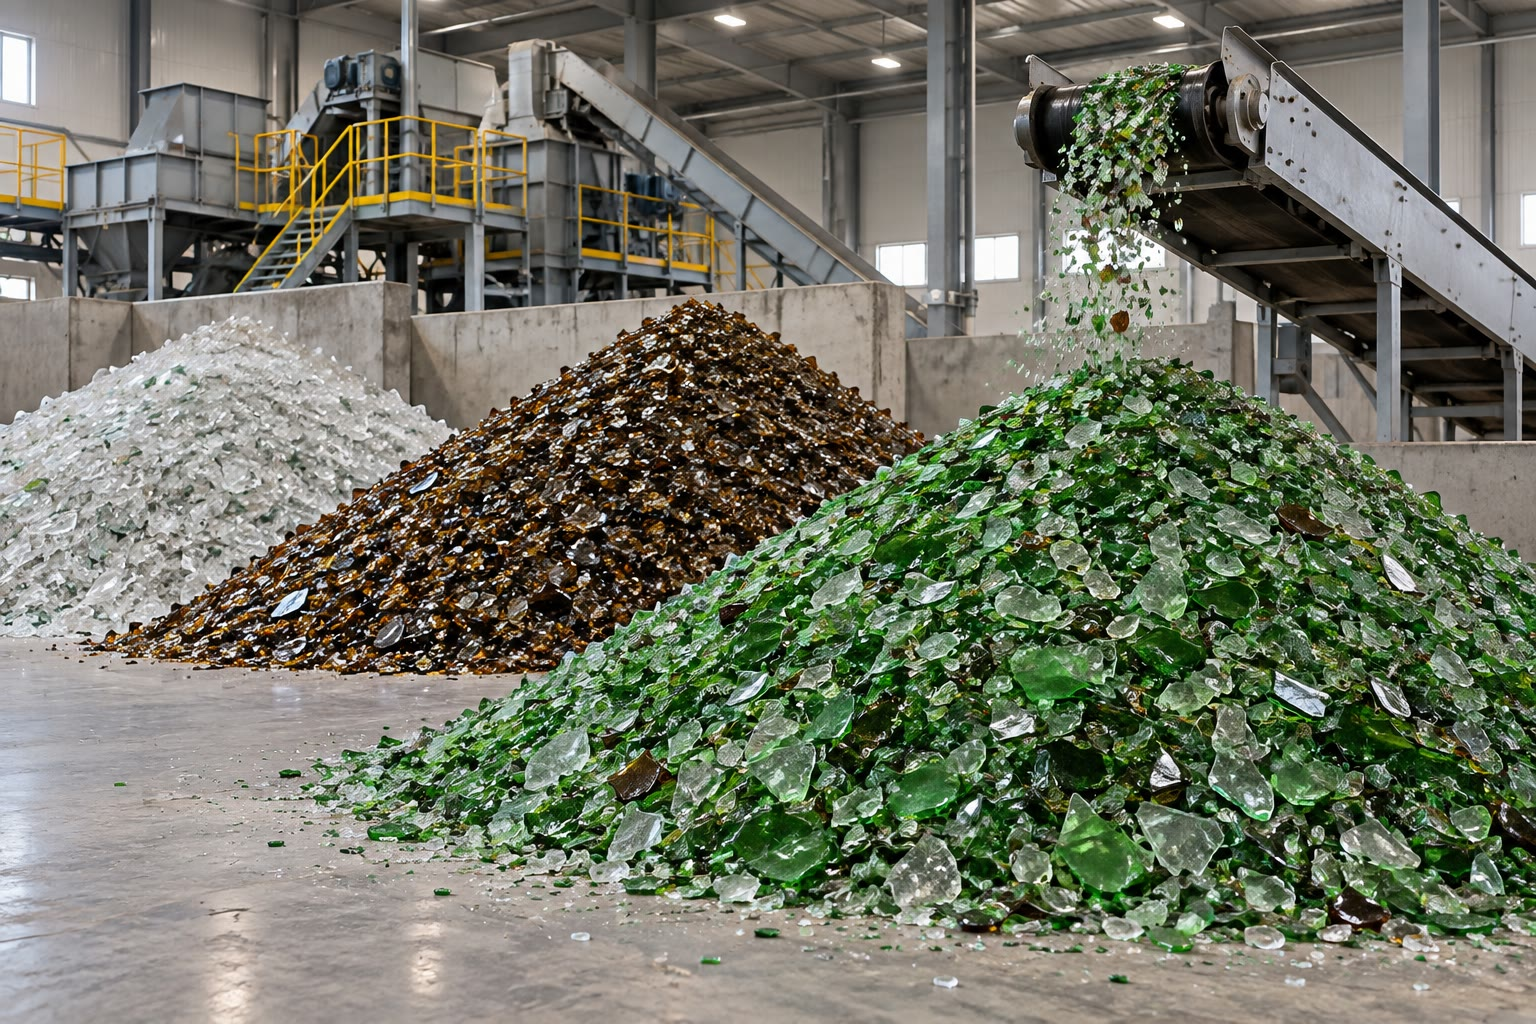
\includegraphics[width=\linewidth,height=4.6cm,keepaspectratio]{images/book1/ai/g5-glass-cullet.jpg}

{\small Vidro moído numa usina de \omterm{def:g5:raw-materials-and-recycling:recycling}{reciclagem}, pronto para ser derretido.}
\end{minipage}\hfill
\begin{minipage}[t]{0.48\linewidth}\centering
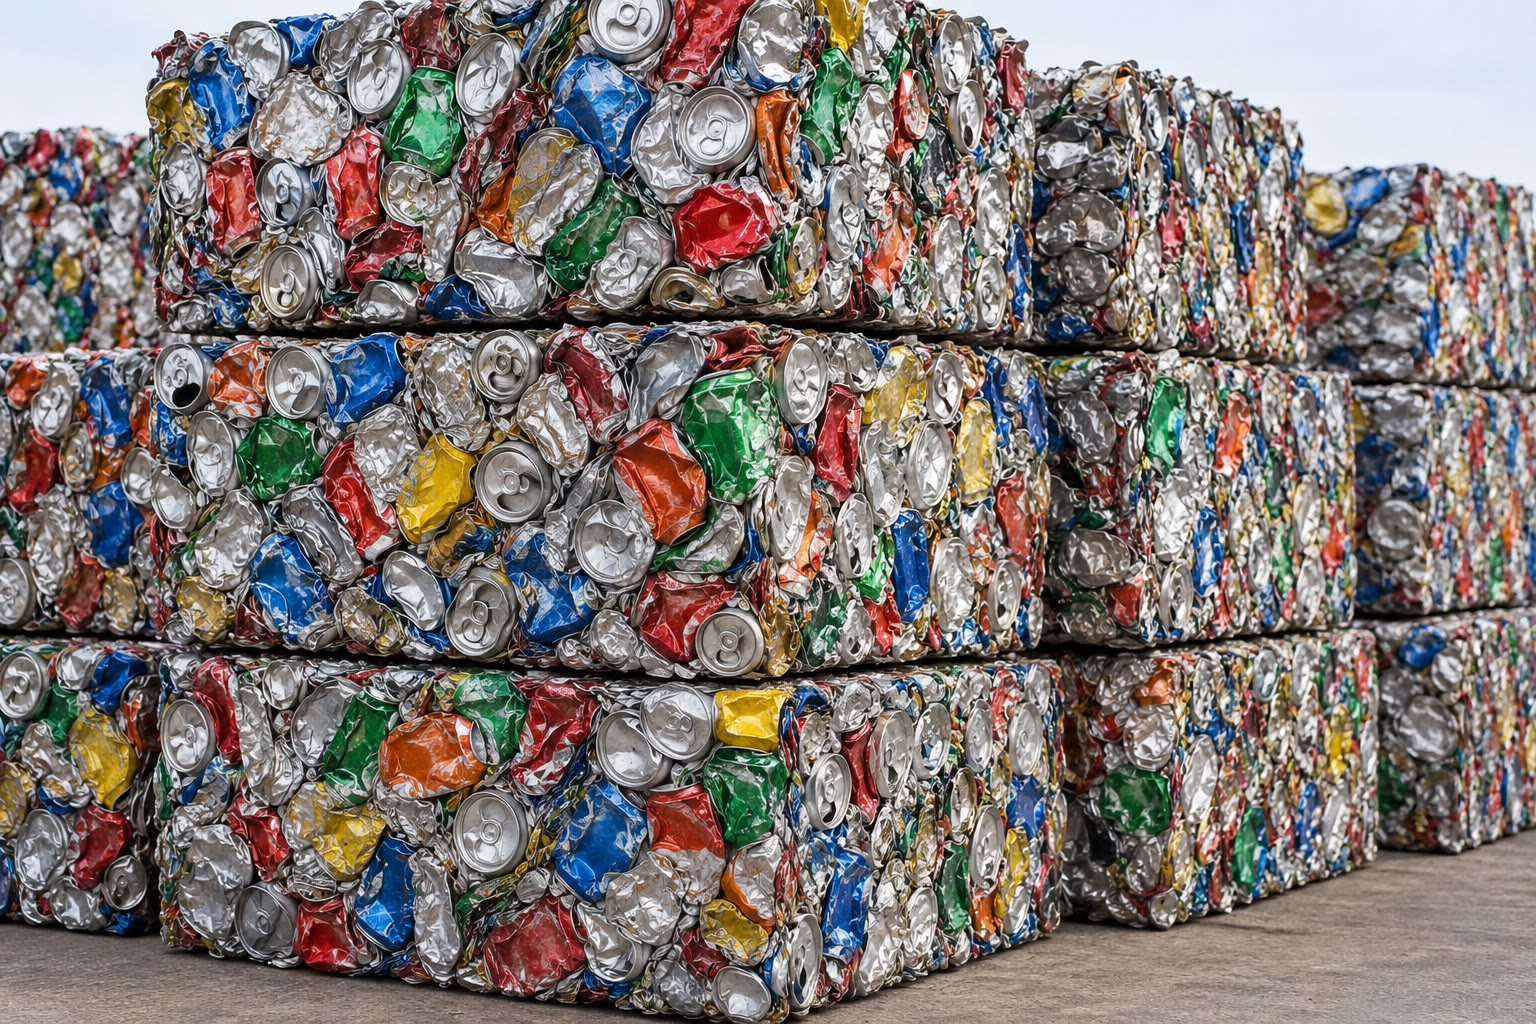
\includegraphics[width=\linewidth,height=4.6cm,keepaspectratio]{images/book1/ai/g5-can-bales.jpg}

{\small Fardos de latinhas de alumínio prensadas.}
\end{minipage}
\end{omfigure}

\section{Lixo e recursos}

\begin{definition}[Recurso]\label{def:g5:raw-materials-and-recycling:resource}
Um \emph{recurso}\index{recurso} é qualquer coisa tirada da natureza que
as pessoas usam: a água, a madeira, os \omterm{def:g5:raw-materials-and-recycling:raw-material}{minérios}, o petróleo, a areia. Um
\emph{recurso renovável}\index{recurso renovavel@recurso renovável} cresce de novo ou volta
sozinho no tempo de uma vida humana, como a madeira de uma floresta que
é replantada ou a lã das ovelhas. Os \omterm{def:g5:raw-materials-and-recycling:raw-material}{minérios} e o petróleo não são
renováveis: depois de extraídos e usados, eles acabam.
\end{definition}

\begin{proposition}[Reduzir, reutilizar, reciclar]\label{prop:g5:raw-materials-and-recycling:three}
Para fazer os \omterm{def:g5:raw-materials-and-recycling:resource}{recursos} durarem, as pessoas podem, nesta ordem:
\begin{enumerate}
  \item \textbf{reduzir}: usar menos objetos, por exemplo menos
        embalagens;
  \item \textbf{reutilizar}: usar de novo o mesmo objeto, como um pote
        de vidro que é enchido outra vez ou uma sacola levada de volta à
        loja;
  \item \textbf{reciclar}: transformar o material num objeto novo.
\end{enumerate}
A \omterm{def:g5:raw-materials-and-recycling:recycling}{reciclagem} vem por último porque ela ainda precisa de energia e de
máquinas; o melhor lixo é o lixo que nunca é produzido.
\end{proposition}

\section{Exercícios}

\begin{exercise}[$\star$]\label{exo:g5:raw-materials-and-recycling:1}
Natural ou fabricado? Madeira, vidro, lã, aço, plástico, pedra.
\end{exercise}

\begin{exercise}[$\star$]\label{exo:g5:raw-materials-and-recycling:2}
Dê a \omterm{def:g5:raw-materials-and-recycling:raw-material}{matéria-prima} de: uma folha de papel, um pote de vidro, uma
camiseta de algodão, uma garrafa de plástico.
\end{exercise}

\begin{exercise}[$\star$]\label{exo:g5:raw-materials-and-recycling:3}
O que é um \omterm{def:g5:raw-materials-and-recycling:raw-material}{minério}? Diga qual é o \omterm{def:g5:raw-materials-and-recycling:raw-material}{minério} do alumínio.
\end{exercise}

\begin{exercise}[$\star$]\label{exo:g5:raw-materials-and-recycling:4}
Em que coletor você põe: um pote de geleia vazio, um jornal, uma
latinha, uma garrafa de plástico de água?
\end{exercise}

\begin{exercise}[$\star$]\label{exo:g5:raw-materials-and-recycling:5}
Olhe a figura da vida de um material. O que o circuito laranja
substitui?
\end{exercise}

\begin{exercise}[$\star$]\label{exo:g5:raw-materials-and-recycling:6}
Renovável ou não: madeira, petróleo, lã, \omterm{def:g5:raw-materials-and-recycling:raw-material}{minério} de ferro, algodão?
\end{exercise}

\begin{exercise}[$\star$]\label{exo:g5:raw-materials-and-recycling:7}
Por que o vidro não pode voltar a ser areia quando é esfriado?
\end{exercise}

\begin{exercise}[$\star$]\label{exo:g5:raw-materials-and-recycling:8}
Dê um jeito de reduzir, um jeito de reutilizar e um jeito de reciclar.
\end{exercise}

\begin{exercise}[$\star$]\label{exo:g5:raw-materials-and-recycling:9}
Por que um coletor de vidro só pode receber vidro?
\end{exercise}

\begin{exercise}[$\star\star$]\label{exo:g5:raw-materials-and-recycling:10}
Produzir alumínio a partir de latinhas velhas exige cerca de um vinte
avos da energia necessária para produzi-lo a partir da bauxita. Uma
fábrica usa 20 unidades de energia para produzir um lote de alumínio a
partir da bauxita. Mais ou menos quantas unidades ela usaria para
produzir o mesmo lote a partir de latinhas velhas?
\end{exercise}

\begin{exercise}[$\star\star$]\label{exo:g5:raw-materials-and-recycling:11}
Por que ``reduzir'' vem antes de ``reciclar''?
\end{exercise}
